\documentclass[conference]{sty/IEEEtran}
\usepackage{times}
\usepackage{wrapfig}
\usepackage{tweaklist}
\usepackage{xspace}
\usepackage{graphicx}
\usepackage{subfigure}
\usepackage{tabularx}
\usepackage{amsmath}
\usepackage{amssymb}
\usepackage{url}
\usepackage{bm}
\usepackage{color}

\def\cH{\mathcal{H}}
\def\cL{\mathcal{L}}
\def\cP{\mathcal{P}}
\def\cO{\mathcal{O}}
\def\mP{{\mathsf P}}
\def\mh{{\mathsf h}}
\def\mo{{\mathsf o}}
\def\mv{{\mathsf v}}
\def\mn{{\mathsf n}}
\def\vcb{{\boldsymbol{c}}}
\def\vpb{{\boldsymbol{p}}}
\def\vqb{{\boldsymbol{q}}}
\def\vnb{{\boldsymbol{n}}}
\def\vlb{{\boldsymbol{l}}}
\def\mr{{\mathsf r}}


% numbers option provides compact numerical references in the text. 
\usepackage[numbers]{natbib}
\usepackage{multicol}
\usepackage[bookmarks=true]{hyperref}

\pdfinfo{
   /Author (Homer Simpson)
   /Title  (Robots: Our new overlords)
   /CreationDate (D:20101201120000)
   /Subject (Robots)
   /Keywords (Robots;Overlords)
}

\begin{document}

% paper title
%\title{Classification of Objects of Daily Use Using Combined Color CHLAC and Global Radius-based Surface Descriptors}
\title{Multidimensional Descriptor for Classification of Objects of Daily Use}

% You will get a Paper-ID when submitting a pdf file to the conference system
\author{Author Names Omitted for Anonymous Review. Paper-ID [add your ID here]}

%\author{\authorblockN{Michael Shell}
%\authorblockA{School of Electrical and\\Computer Engineering\\
%Georgia Institute of Technology\\
%Atlanta, Georgia 30332--0250\\
%Email: mshell@ece.gatech.edu}
%\and
%\authorblockN{Homer Simpson}
%\authorblockA{Twentieth Century Fox\\
%Springfield, USA\\
%Email: homer@thesimpsons.com}
%\and
%\authorblockN{James Kirk\\ and Montgomery Scott}
%\authorblockA{Starfleet Academy\\
%San Francisco, California 96678-2391\\
%Telephone: (800) 555--1212\\
%Fax: (888) 555--1212}}


% avoiding spaces at the end of the author lines is not a problem with
% conference papers because we don't use \thanks or \IEEEmembership


% for over three affiliations, or if they all won't fit within the width
% of the page, use this alternative format:
% 
%\author{\authorblockN{Michael Shell\authorrefmark{1},
%Homer Simpson\authorrefmark{2},
%James Kirk\authorrefmark{3}, 
%Montgomery Scott\authorrefmark{3} and
%Eldon Tyrell\authorrefmark{4}}
%\authorblockA{\authorrefmark{1}School of Electrical and Computer Engineering\\
%Georgia Institute of Technology,
%Atlanta, Georgia 30332--0250\\ Email: mshell@ece.gatech.edu}
%\authorblockA{\authorrefmark{2}Twentieth Century Fox, Springfield, USA\\
%Email: homer@thesimpsons.com}
%\authorblockA{\authorrefmark{3}Starfleet Academy, San Francisco, California 96678-2391\\
%Telephone: (800) 555--1212, Fax: (888) 555--1212}
%\authorblockA{\authorrefmark{4}Tyrell Inc., 123 Replicant Street, Los Angeles, California 90210--4321}}

\newcommand{\todo}[1]{\textbf{\textcolor{red}{TODO: #1}}}
\maketitle

\begin{abstract}
The abstract goes here.

\end{abstract}

\IEEEpeerreviewmaketitle

\section{Introduction}
One of the great challenges faced by autonomous mobile robot
manipulation is the scaling of the technology to realistic tasks, in
realistic environments under realistic conditions. This challenge
implies that an autonomous household robot is required to act on many
different objects of daily use, to handle them in typical situations
for example when opening a fridge to get the milk or when performing
realistic tasks such as setting the table or preparing a meal.

\begin{figure}[htb!]
  \begin{center}
    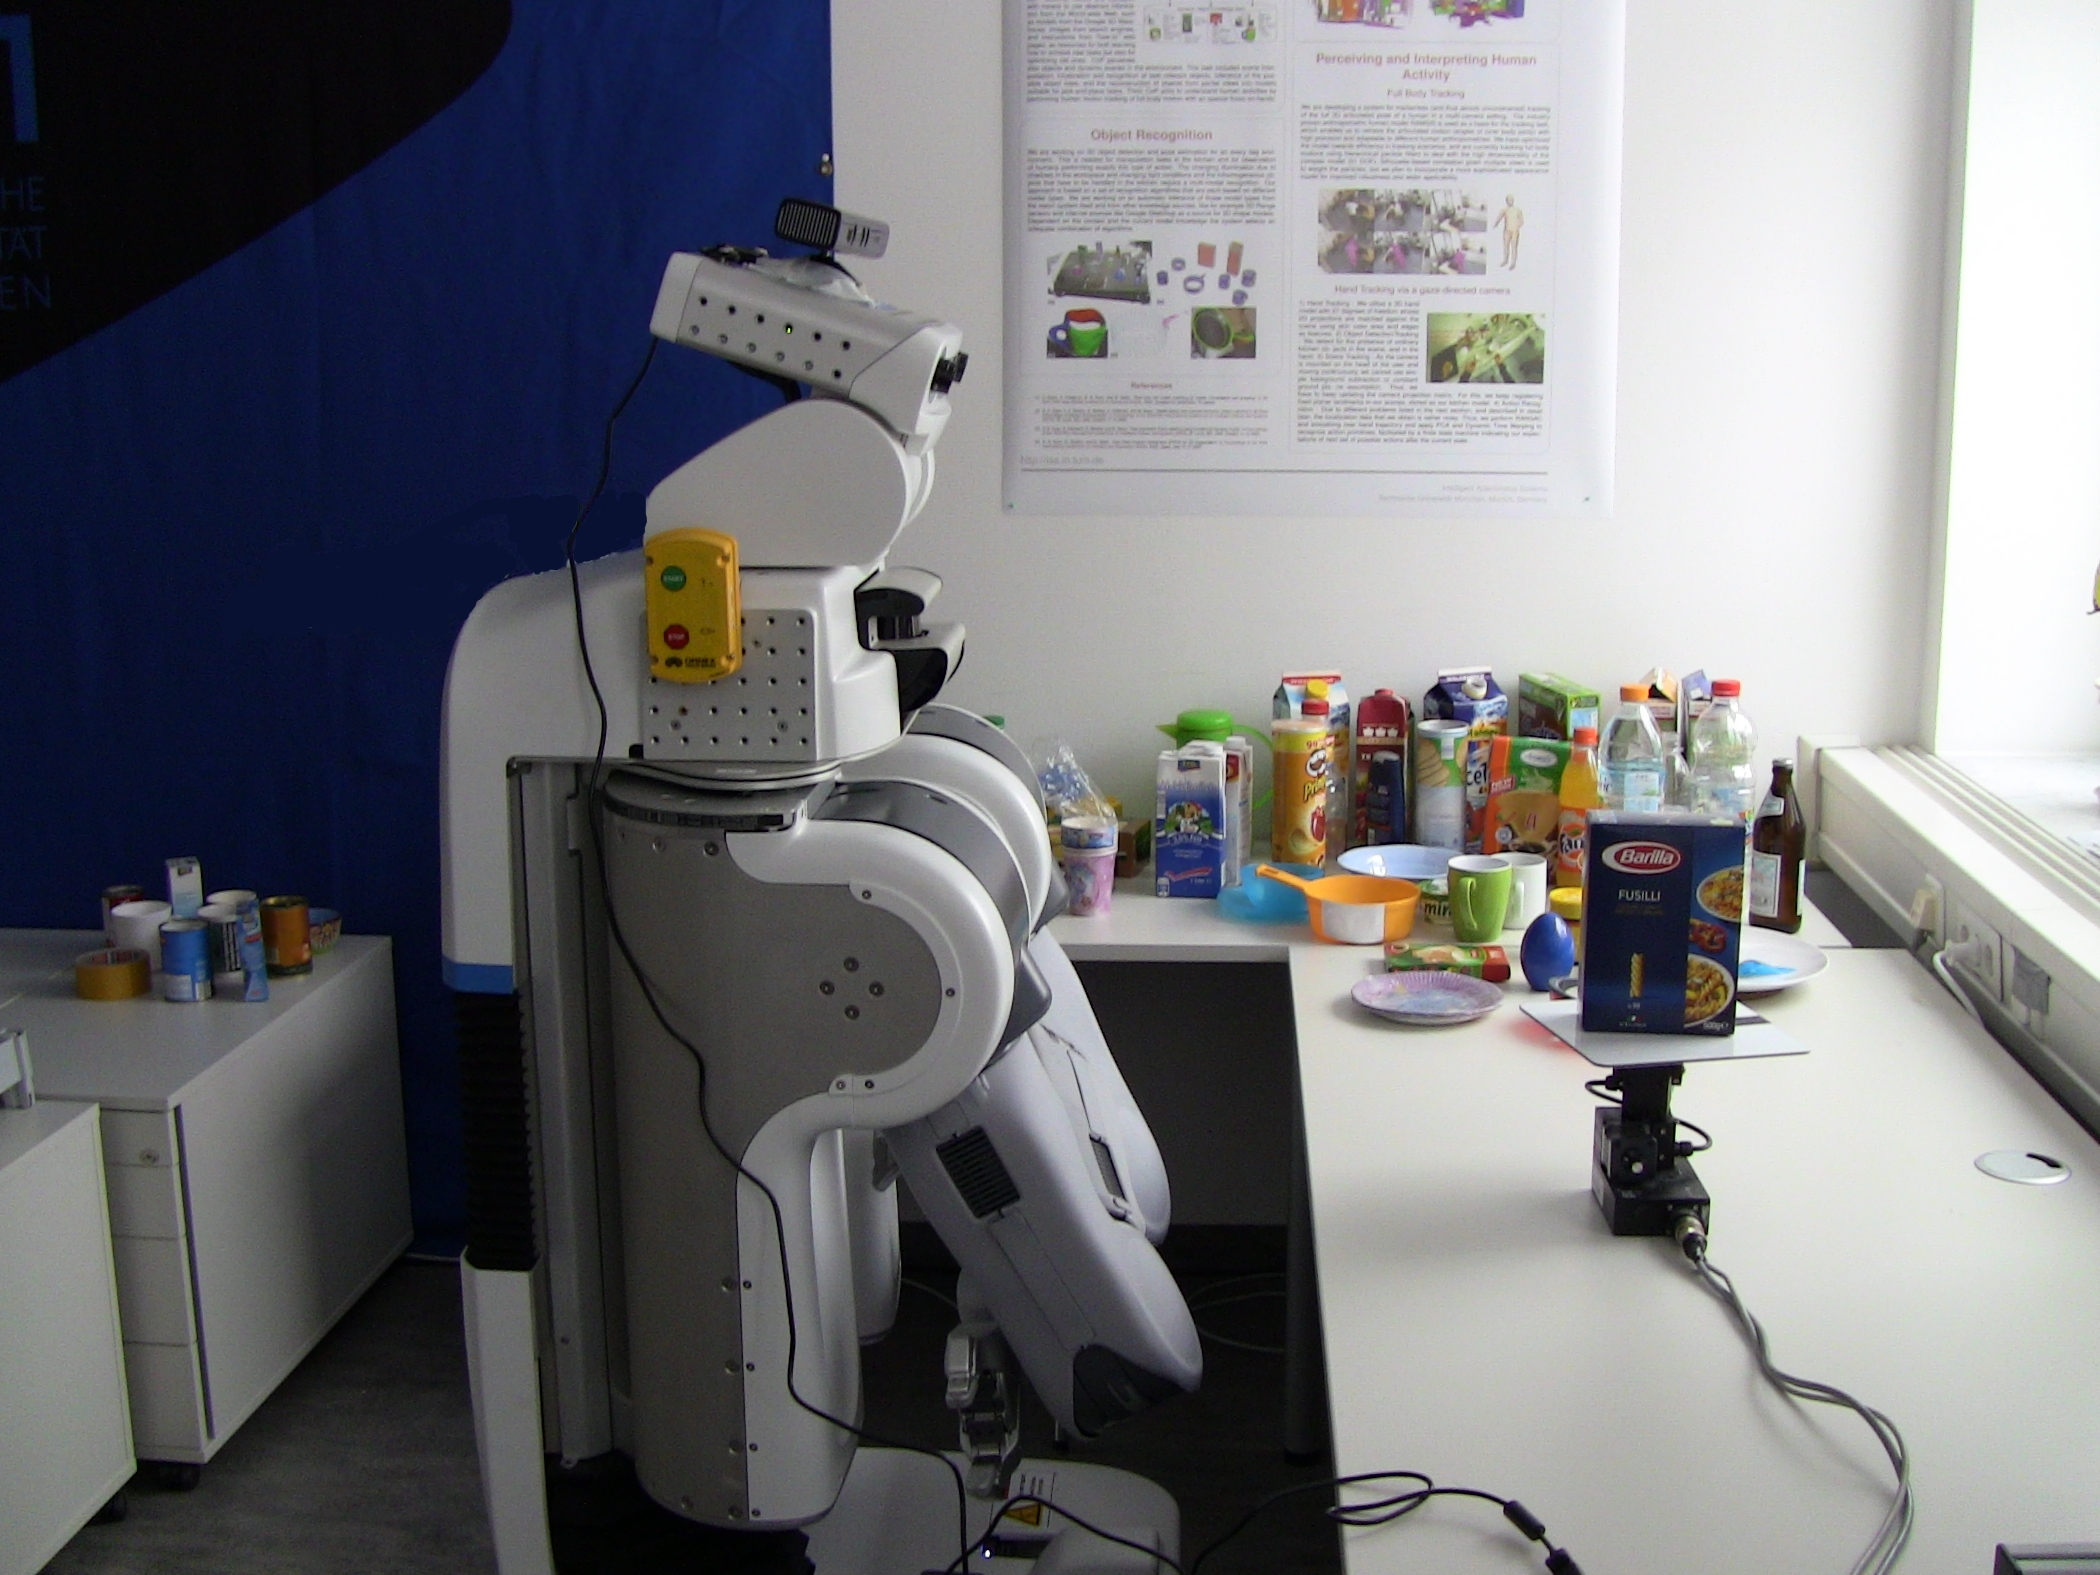
\includegraphics[width=.9\columnwidth]{figures/objects/pr2_rot_table.jpg}
    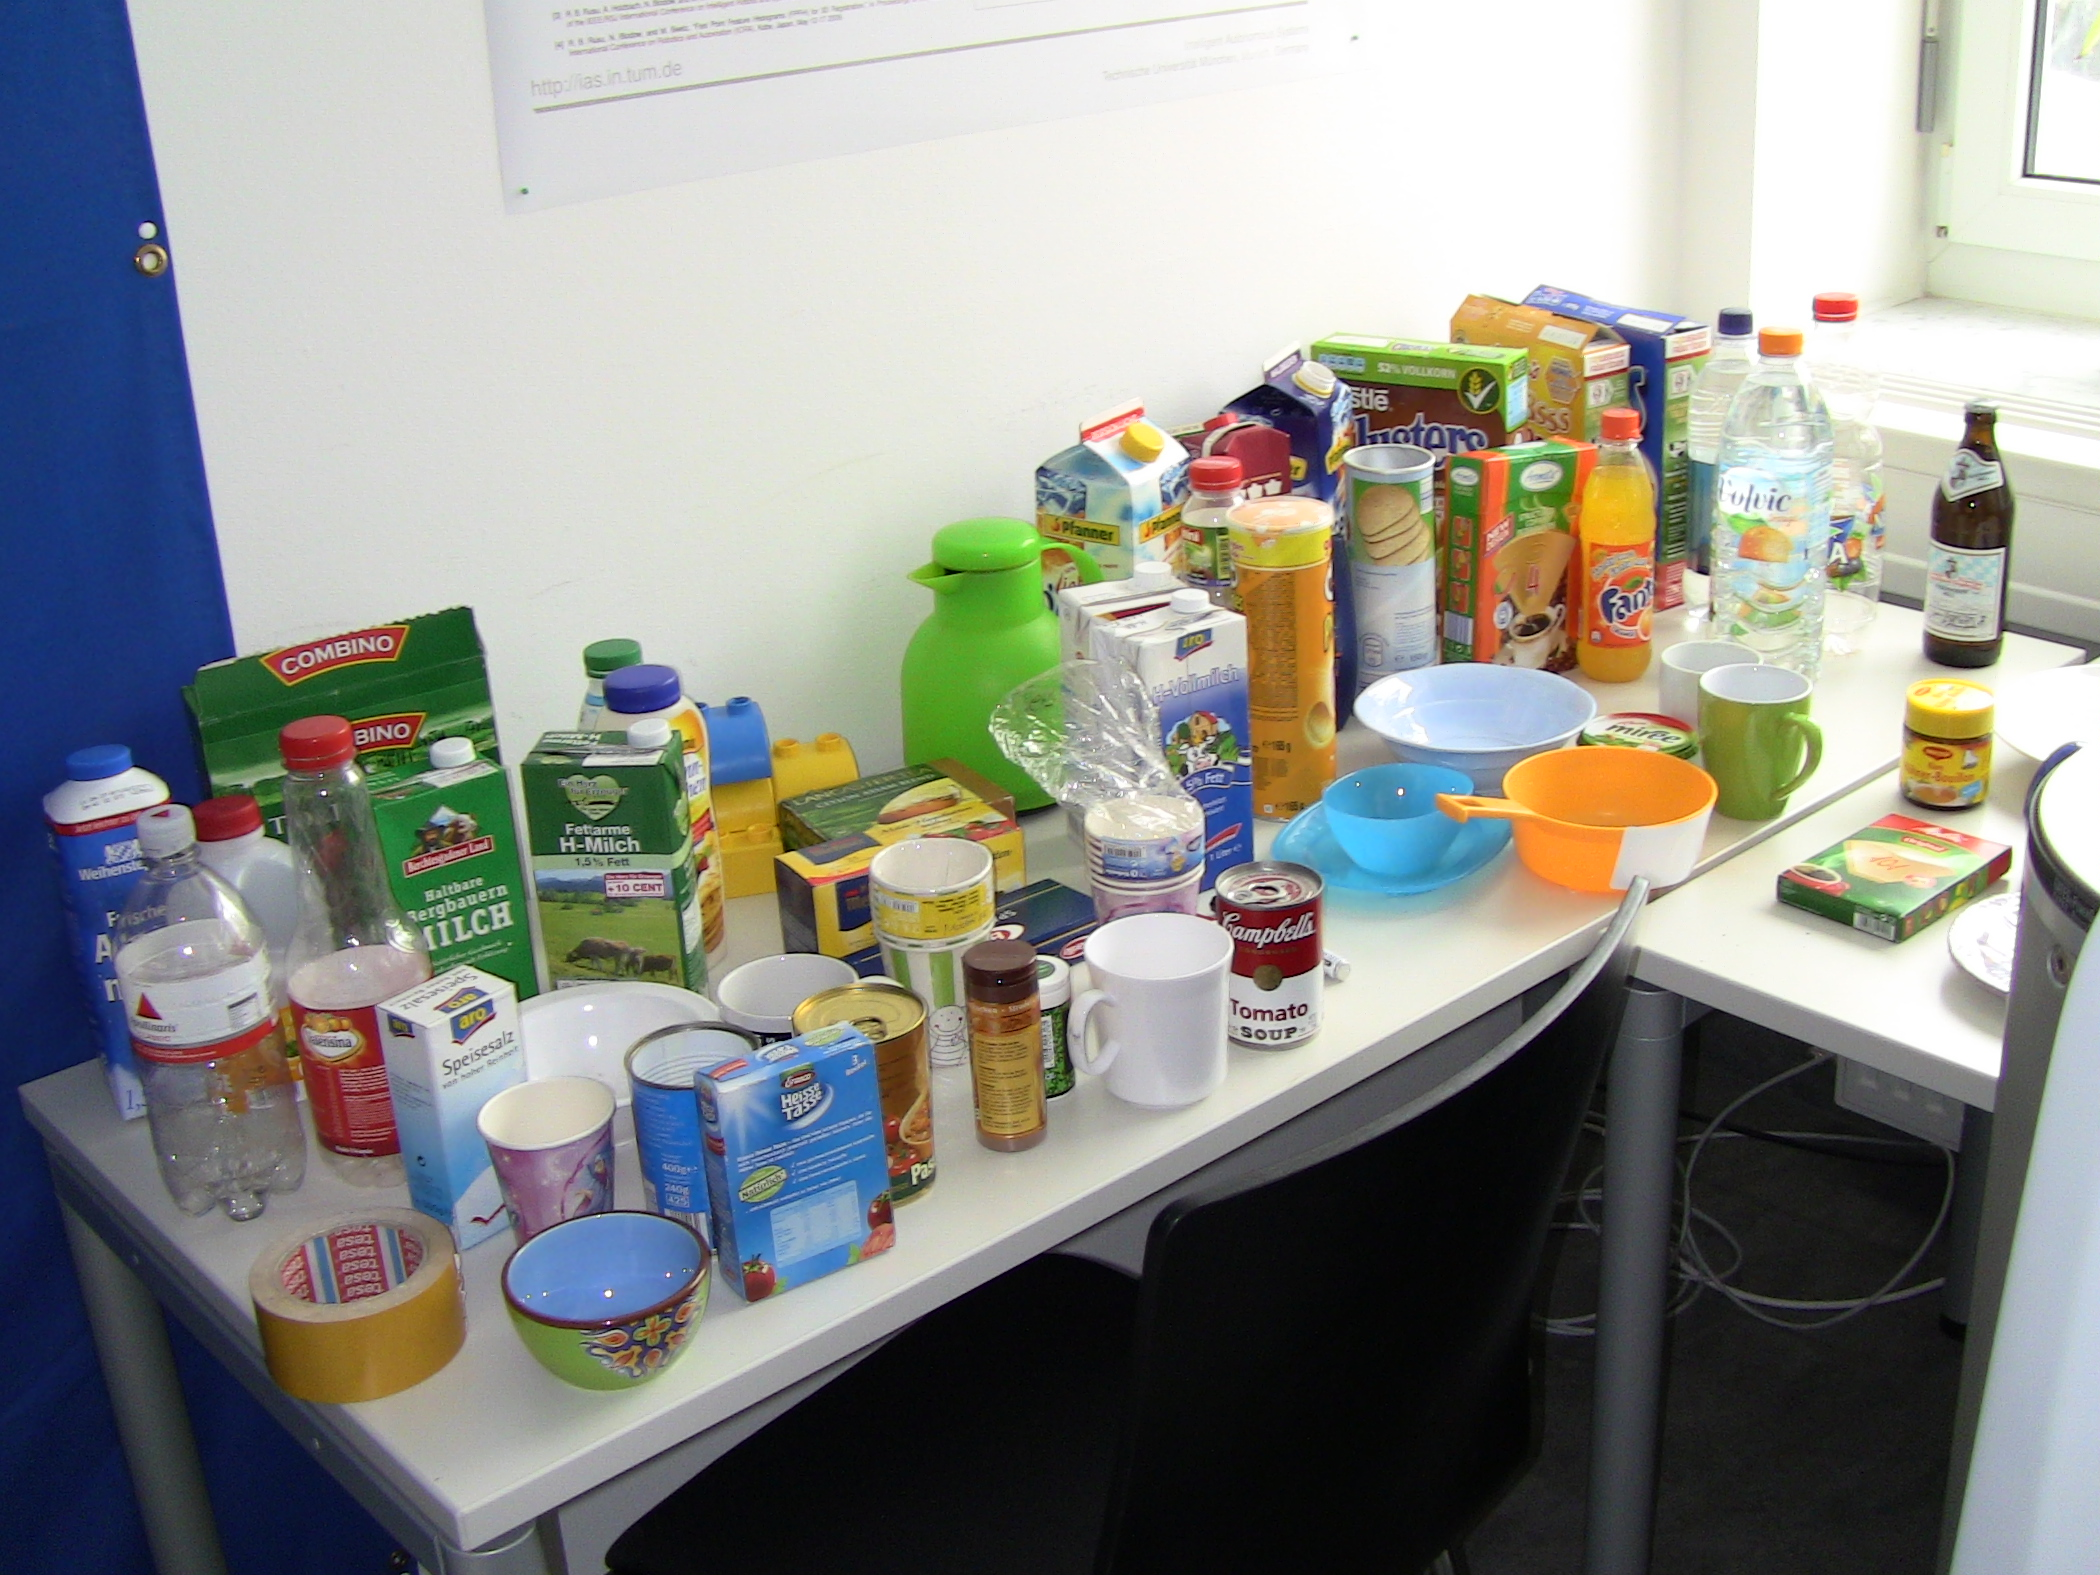
\includegraphics[width=.9\columnwidth]{figures/objects/objects.jpg}
    \caption{Top: an autonomous service robot PR2 with a mounted Kinect sensor
    acquiring training data of the objects shown in bottom part of Figure}
    \label{fig:robot}
  \end{center}
\end{figure}

\subsection{What}
The problem Problem statement:
\begin{itemize}
\item Recogniton and localization of objects of daily use in households
\item Categorization and classification with \emph{one} descriptor
\item Omits a supporting-table assumption and performs in cluttered and occluded scenes
\item Runs online
\end{itemize}


\subsection{Why}
\begin{itemize}
\item to equipp the service robots with the boostrapped recognition models and capabilities
to acquire additional models
\item to enable manipulation tasks in realistic environments under realistic conditions
\item to exploit new sensing technology (e.g. Kinect) and to thus avoid decoupling of gemetrical and
visual appearance data
\end{itemize}


\subsection{How}
\begin{itemize}
\item Combination of view-variant ColorCHLAC and GRSD with the
normalization of the latter by number 27 (number of transitions)
\item Combination of view-invariant version of ColorCHLAC and GRSD
\item Comparisson of Linear Subspace Method and SVM Classifier
\end{itemize}

\subsection{Novelty}

The remainder of the paper is built as following. After the overview of the related
work in Section~\ref{sec:rl} we present the major system components in Section~\ref{sec:overview}
which is followed by Section~\ref{sec:features} that elaborates on the construction of the
GRSDColorCHLAC descriptor. In Section~\ref{sec:classification} we present the usage of this descriptor
for the classification of objects using two state-of-the-art classification methods which we
then elaborately test and present in Section~\ref{sec:results}. In Section~\ref{sec:conclusion}
we conclude and give the future outlook.

\section{Related Work}
\label{sec:rl}
\begin{itemize}
\item VFH~\cite{vfh}
\item GRSD (Humanoids10GRSD~)\cite{GRSD10Humanoids}
\item Color CHLAC (Asako)~\cite{kanezaki2010icra}\cite{kanezaki2010tvc}
\item NARF~\cite{steder10irosws}
\item textured-spin images~\cite{Johnson_spin_images}
\item SIFT~\cite{Lowe04distinctive}
\item A sparse texture representation using local affine regions~\cite{Lazebnik05asparse}
\item sift-keypoint \url{http://www.ros.org/doc/api/pcl/html/sift__keypoint_8h_source.html}
\item Combining Depth and Color Cues for Scale and Viewpoint-Invariant
Object Segmentation and Recognition Using Random Forests - the emphasize is on classifier Random Forests~\cite{stueckler10combining}
\end{itemize}

\section{System Overview} 
\label{sec:overview}
\todo{Dejan}

\section{Feature Estimation}
\label{sec:features}

\subsection{Color CHLAC}
\todo{Asako - explain the difference between viewpoint variant and invariant}\\
Color-CHLAC features are computed from color 3D voxel data by measuring 
    the autocorrelation function of the 3D target object at specific points, 
    represented by local patterns.
Local descriptors are represented by correlation values of the colors of neighboring voxels.

Letting $\bm{x}=(x,y,z)^T$ be the position of a voxel, 
    we use the notation $p(\bm{x})=1$ if the voxel is occupied, and $p(\bm{x})=0$ otherwise. 
When $p(\bm{x})=1$, the voxel has RGB color values.
We represent them as $r(\bm{x})$, $g(\bm{x})$ and $b(\bm{x})$, 
    which are normalized between 0 and 1.
By defining $r'(\bm{x}) \equiv 1 - r(\bm{x})$, $g'(\bm{x}) \equiv 1 - g(\bm{x})$ and $b'(\bm{x}) \equiv 1 - b(\bm{x})$, 
    a voxel status $\bm{f}(\bm{x})\in R^6$ is defined as follows:
%\vspace{-2mm}
\begin{eqnarray*}
  \label{eq:voxel}
%  \hspace{-1mm}
  \bm{f}({\bm x})\hspace{-1mm}=\hspace{-1mm}\left\{
  \begin{array}{cc}
    \hspace{-1mm}
    (r({\bm x})\hspace{1mm} r'({\bm x}) \hspace{1mm}g({\bm x}) \hspace{1mm}g'({\bm x}) \hspace{1mm}b({\bm x}) \hspace{1mm}b'({\bm x}))^T & \hspace{-2mm}(p({\bm x})\hspace{-1mm}=\hspace{-1mm}1) \\
    (0\hspace{1mm}0\hspace{1mm}0\hspace{1mm}0\hspace{1mm}0\hspace{1mm}0)^T & \hspace{-2mm}(p({\bm x})\hspace{-1mm}=\hspace{-1mm}0)
  \end{array}\right.
\end{eqnarray*}
%
Color-CHLAC features are the integral of $\bm{f}(\bm{x})$ or correlations of $\bm{f}(\bm{x})$ between neighboring voxels.
They are calculated by following equations:  
\begin{equation}\label{eq:0th}
  {\bm q} = \int \bm{f}({\bm x}) d{\bm x} 
\end{equation}
%\vspace{-4mm}
\begin{equation}\label{eq:1st}
  {\bm q}({\bm a}) = \int \bm{f}({\bm x}) \hspace{1mm}\bm{f}^T({\bm x}+{\bm a}) d{\bm x} \\
\end{equation}
%
The dimension of Color-CHLAC features calculated by (\ref{eq:0th}) is 6. 
14 patterns are used for the displacement vectors ${\bm a}$ in (\ref{eq:1st}) (Fig. \ref{fig:displacement_vectors}). 
Note that not only $\bm{f}(\bm{x})$ correlation between two neighboring voxels 
    but also the correlation between two elements of $\bm{f}(\bm{x})$ of one voxel is integrated. 

\begin{figure}[htb!]
  \begin{center}
    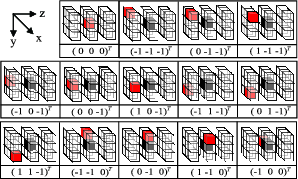
\includegraphics[width=0.43\textwidth]{figures/colorCHLAC/displacement_vectors.png}
    %\vspace{-2mm}
    \caption{Patterns of displacement vectors. Position of the center voxel is ${\bm x}$, 
      while position of the other highlighted voxel is ${\bm x}+{\bm a}$. }
    \label{fig:displacement_vectors}
  \end{center}
\end{figure}

As a pre-processing of features extraction, $r(\bm{x})$, $g(\bm{x})$ and $b(\bm{x})$ can be binarized. 
Excluding redundant elements, the dimension of Color-CHLAC features calculated by (\ref{eq:1st}) is 
    480 if color values are binarized, and 489 otherwise.
In this paper, we extract Color-CHLAC features both from binarized color voxel data and from original color voxel data. 
Then the dimension of Color-CHLAC feature vector becomes 981 (=6+480+6+489). 


\subsection{GRSD}
%
GRSD is a histogram, that counts the number of transitions between different types of voxels.
This approach is similar to ColorCHLAC, but in order to efficiently merge the two features,
the original GRSD has to be simplified. As presented in \cite{GRSD10Humanoids} we were using
ray-tracing in order to find transitions between surface types of voxels. To merge the features,
ray-tracing was abandoned for simple checks of neighboring voxels, and the feature is no longer normalized.

These modifications allow us to create histograms which, like ColorCHLAC, are roughly additive.
If we break up objects into reasonable sizes, its histogram can be approximated by the sum of the
histograms of its partitioning. Unlike in ColorCHLAC, free space is considered, but we are looking
at the neighbors of occupied voxels only.

As the feature is rotation invariant, the number of bins $b$ depends on the number of possible surface types $s$ (including emph-empty):
\begin{equation}
b=\frac{s(s+1)}{2}-s
\end{equation}
Previously only predefined surface types with an intuitive description were used (cylinder, sphere, plane, rim and corner),
based on an estimation of the radii of the 2 principal curves defining the surface, $r_{min}$ and $r_{max}$ \cite{Marton10IROS}.
Since these values have physical meaning, we can categorize surfaces into predefined types, but 
\todo{now we are dividing, so we get more surface types, chosen to roughly match ColorCHLAC to have the same "weighting"}

\begin{figure}[htb!]
  \begin{center}
    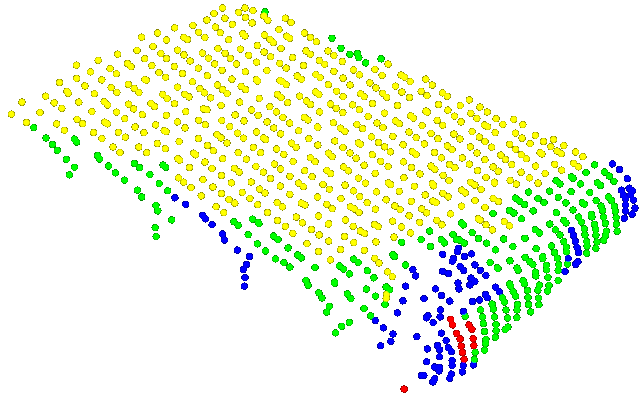
\includegraphics[width=.4\columnwidth]{figures/grsd/book.png}
\hfill
    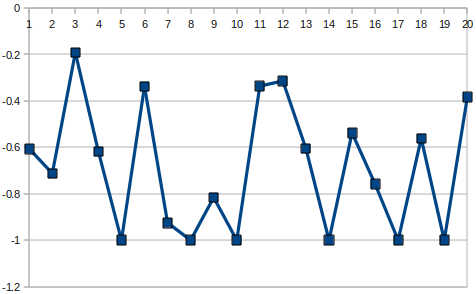
\includegraphics[width=.48\columnwidth]{figures/grsd/book_global.png} \\
\hfill
    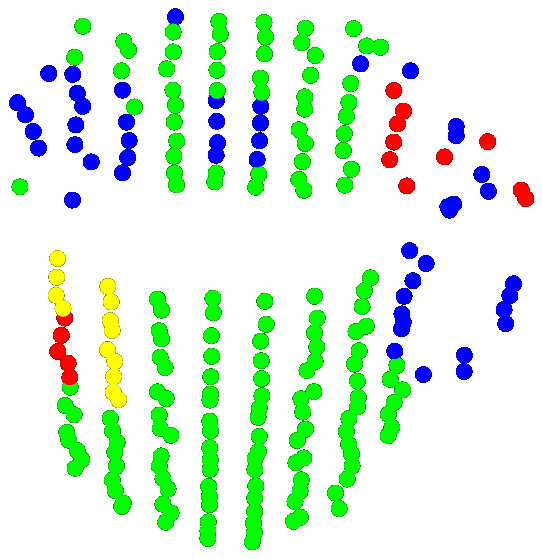
\includegraphics[width=.3\columnwidth]{figures/grsd/mug.png}
\hfill
    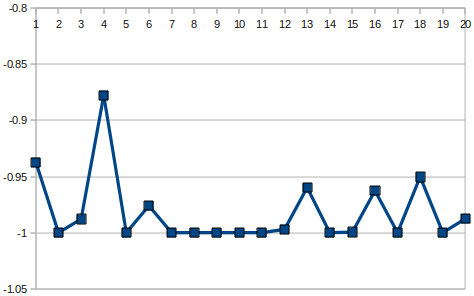
\includegraphics[width=.48\columnwidth]{figures/grsd/mug_global.png}
\caption{Example of RSD classes and GRSD plots for a big flat box (i.e. book, upper row) and a short cylinder (i.e. mug, bottom row).
The histogram bin values are scaled between -1 and 1 according to the
training data, and the colors represent the following local surfaces:
red - sharp edge (or noise), yellow - plane, green - cylinder, light blue -
sphere (not present), and dark blue - rim (i.e. boundary, transition between surfaces).
\emph{Best viewed in color.}
}
    \label{fig:gfpfh}
  \end{center}
\vspace{-2ex}
\end{figure}

Once all voxels are annotated locally using a geometric class, our
processing pipeline constructs a global feature by counting the transitions
between these local labels (and free space), as shown in Figure~\ref{fig:gfpfh}.
Since we do not use ray-casting but consider only the direct neighbors
of each occupied cell, the computation of this \emph{simplified} GRSD is much faster.

\begin{figure}[htb!]
  \begin{center}
    \includegraphics[width=.48\columnwidth]{figures/colorCHLAC/artificial/purple.png}
    \includegraphics[width=.48\columnwidth]{figures/colorCHLAC/artificial/torus.png}
    \caption{Examples of GRSD-ColorCHLAC histograms. Left: different categories 
of objects result in having different first 20 bins of the respective histogram.
Right: different colors of the same category of an object have different 117 last bins 
of the histogram}
    \label{fig:grsd_cchlac}
  \end{center}
\end{figure}

\subsection{Comparison}
%
Same approach (if using rotation invariant ColorCHLAC), but different things are counted (color vs surface type). Also, GRSD considers free space as well.
\begin{figure}[htb!]
  \begin{center}
    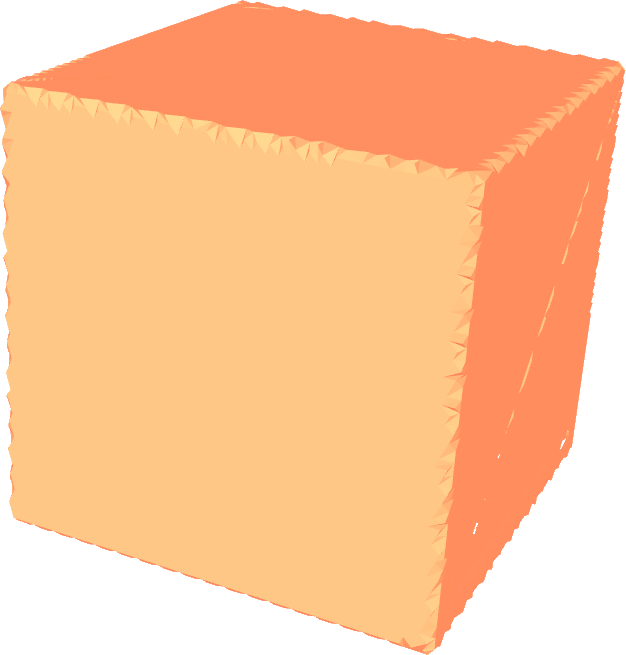
\includegraphics[width=.3\columnwidth]{figures/comparison/cube.png}
    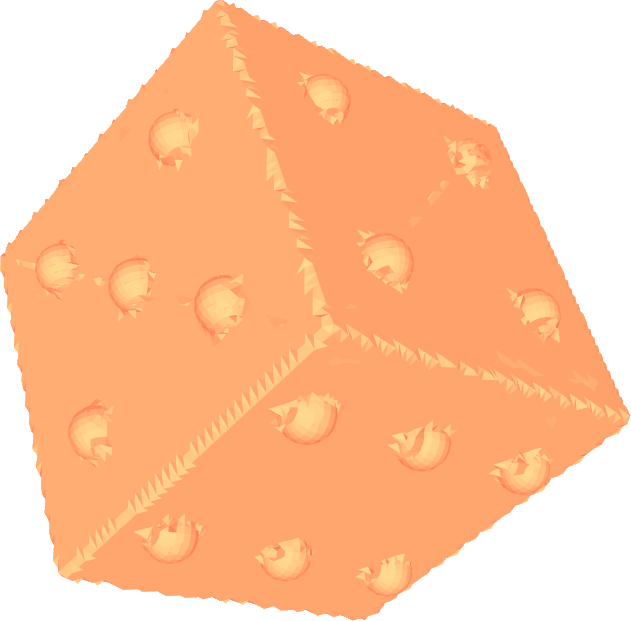
\includegraphics[width=.32\columnwidth]{figures/comparison/dice1.png}
    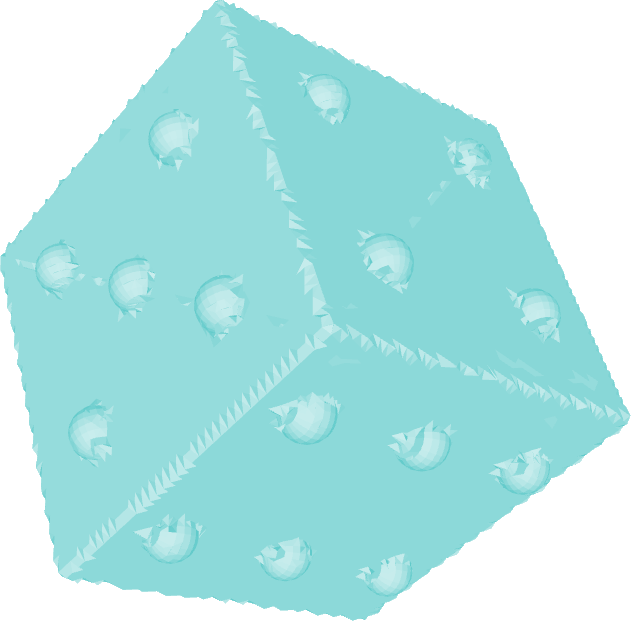
\includegraphics[width=.32\columnwidth]{figures/comparison/dice2.png}
    \caption{Color-CHLAC: can not differentiate the dice from the cube. GRSD: can not differentiate the different colors. Combination solves both.}
    \label{fig:comparison}
  \end{center}
\vspace{-2ex}
\end{figure}

\section{Classification Methods}
\label{sec:classification}
\subsection{Linear Subspace Method}
\label{sec:subspace}
\subsubsection{Creating subspaces of objects in a database}
First, the voxel data of each object in a database is subdivided into a voxel grid of a certain size, 
    e.g. $10 \times 10 \times 10$ voxels. 
Suppose the $i$-th object in the database is divided into $M_i$ subdivisions.
Then $M_i$ Color-CHLAC feature vectors are extracted. 
To achieve robustness to rotation, 
    features extraction is repeated with various poses of the object. 
The feature vector of an object which is rotated by 90 degrees can be obtained rapidly
    through a simple exchange of the elements of the feature vector in the initial posture.
This is possible because each displacement vector in Fig.~\ref{fig:displacement_vectors}
    is equivalent to another, rotated by 90 degrees.
In this paper, we use this 90 degrees rotation in 24 ways,
    and rotations of 30 and 60 degrees in 21 ways, 
    resulting in achieving 504($=24 \times 21$) varieties of postures for an object. 
Therefore, the number of Color-CHLAC feature vectors 
    generated from each object is $N_i \equiv 504M_i$. 

We represent a Color-CHLAC feature vector compressed by PCA as $\bm{z}_t \in R^d, t=1,2,...N_i$, 
    where $d$ is the dimension of a compressed feature vector.
The auto-correlation matrix of these feature vectors is calculated by the following equation: 
\begin{eqnarray*}
  %\hspace{-1mm}
  R_i = \frac{1}{N_i} \sum^{N_i}_{t=1} \bm{z}_t \bm{z}_t^T
\end{eqnarray*}
The eigenvectors of $R_i$ are then computed by solving the eigenvector problem. 
Finally, the bases of the subspace of the $i$-th object in the database, $P_i \equiv (\bm{v}_{i1} \bm{v}_{i2} ... \bm{v}_{ir})$, 
    are obtained as the $r$ eigenvectors of largest eigenvalue. 

\subsubsection{Calculation of Similarity}
The first step in the recognition process is to compute 
    one Color-CHLAC feature vector from the whole of a query part in a 3D scene. % ???
Then the compressed feature vector $\bm{z}$ is computed using the projection matrix which is 
    generated from all Color-CHLAC feature vectors of each database object in the pre-processing phase.
Let the similarity between the query part and the $i$-th object in the database be $y_i$. 
$y_i$ is defined as the cosine of the angle between $\bm{z}$ and the subspace of the $i$-th object.
$y_i$ is calculated by the following equation: 
\begin{eqnarray}\label{eq:y_calc}
  %\hspace{-1mm}
  y_i = \frac{\| P_i^T \bm{z} \|}{\| \bm{z} \|}
\end{eqnarray}


\subsection{Support Vector Machine-based Classification}
\todo{Zoli}

\section{Results}
\label{sec:results}
\subsection{Data Acquisition and Training}
Our database of 3D objects, available at \url{http://semantic-3d.cs.tum.edu},
(\todo{upload}) was obtained using the Kinect sensor. 

The set of objects (see Figure~\ref{fig:robot}) encompasses the ones commonly used 
in a typical household environment (mugs, utensils, books, etc) and is envisioned for a
larger expansion in the future.  In a pursue to account for a wide variety
of view angles, we rotated the objects on the rotating table with a given
angle-step ($15^\circ$ in the preliminary version) and acquired partial
snapshots from a human-eye perspective, i.e. the ones that the best
approximate the robot's view point during its working cycle.  We consider
this to be an important point as opposed to similar initiatives (e.g.,
\cite{kit}) where the datasets are acquired using high-precision but
non-affordable, fixed sensors, and thus not usable for applications such as ours.

\begin{figure}[htb!]
  \begin{center}
    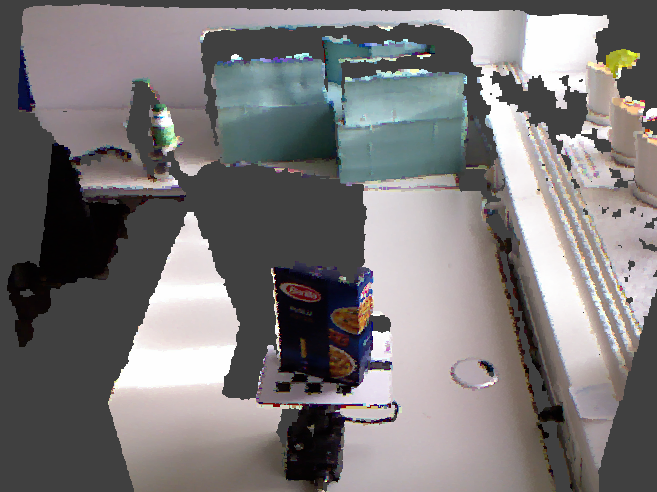
\includegraphics[width=.45\columnwidth]{figures/rot_table/barilla.png}
\hfill
    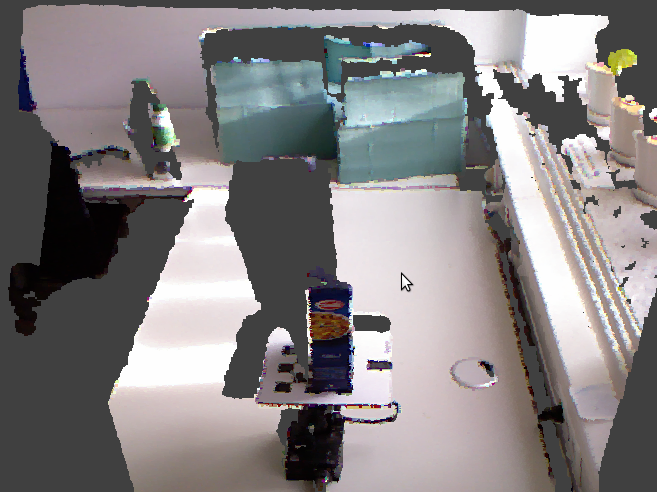
\includegraphics[width=.45\columnwidth]{figures/rot_table/barilla1.png} \\
    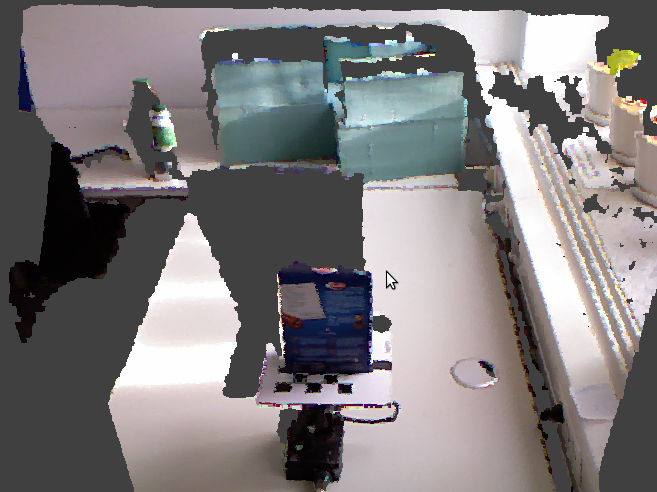
\includegraphics[width=.45\columnwidth]{figures/rot_table/barilla2.png}
\caption{Acquisition of Training Data}
    \label{fig:data_acquisition}
  \end{center}
\end{figure}

\subsection{Testing}
\begin{figure}[htb!]
  \begin{center}
    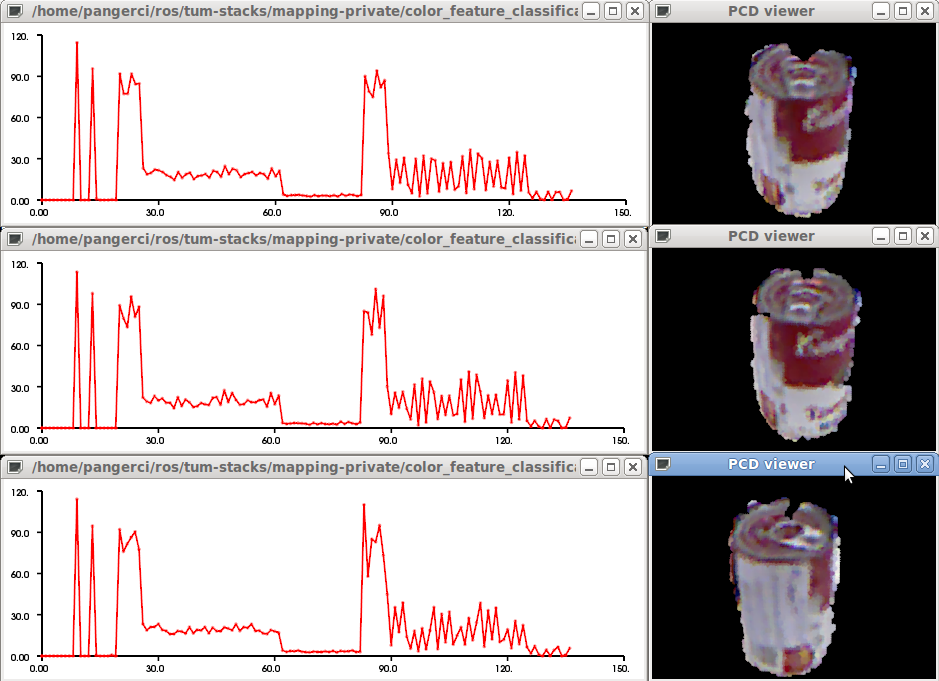
\includegraphics[width=.9\columnwidth]{figures/colorCHLAC/real/tomato/tomato_hist_pcd.png}
    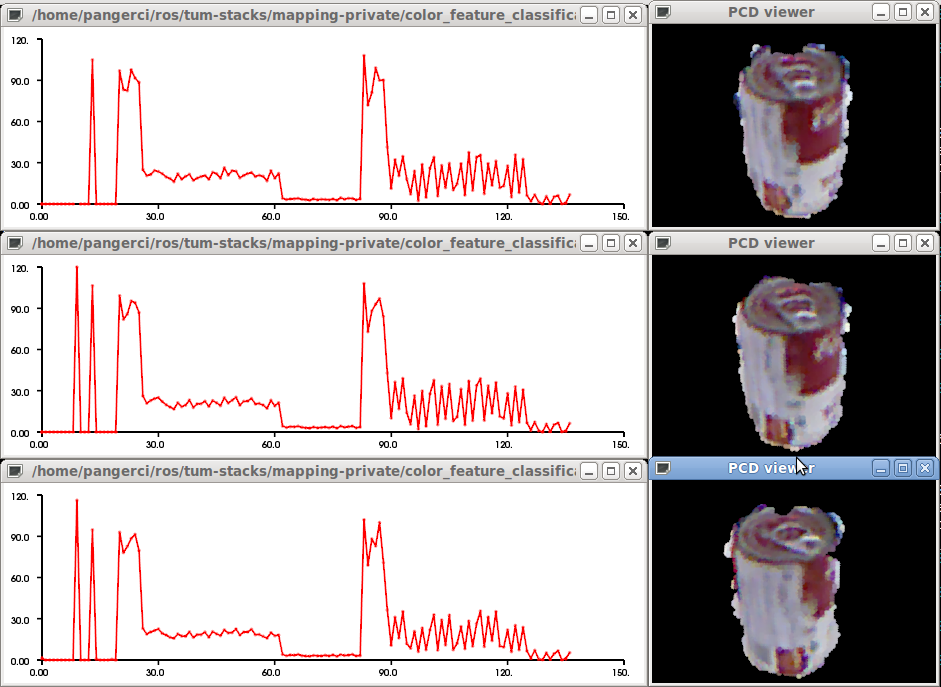
\includegraphics[width=.9\columnwidth]{figures/colorCHLAC/real/tomato/tomato_hist_pcd2.png}
    \caption{Examples of GRSD-ColorCHLAC histograms for a Tomato Soup can.}
    \label{fig:grsd_colorchlac_tomato}
  \end{center}
\end{figure}

\subsubsection{Cross-Validation}
\todo{ALL}

\subsubsection{Find One Object Test}

\todo{Dejan}

\subsection{Object Recognition Pipeline (in Clutter)}
We applied our object recognition method on an object detection scheme in a cluttered environment. 
The system computes the similarities between each target object and all recutangular-solid sub-regions in the environment, and then it outputs all the regions that have higher similarities than a certain threshold as the candidates of the target object.
Each sub-region has the same size as that of the bounding box of the target object. 
To accelerate feature extraction from the sub-regions, we used ``Integral Feature Table''~\cite{kanezaki2010tvc}, which is a simple extention of ``Integral Image''~\cite{viola2001} from 2D to 3D.
The ``Integral Feature Table'' $\bm{I}(x,y,z)$ is defined as the $d$-dimensional compressed feature vector extracted from the voxel area 
    ranging from $(0,0,0)$ to $(x,y,z)$.
Let the feature vector of the voxel area with $x$ ranging from $x_1$ to $x_2$, 
    $y$ ranging from $y_1$ to $y_2$, and $z$ ranging from $z_1$ to $z_2$, be $\bm{F}(x_1,y_1,z_1,x_2,y_2,z_2)$. 
This is computed by the following equation: 
\begin{eqnarray*}\label{eq:sat}
\bm{F}(x_1,y_1,z_1,x_2,y_2,z_2) = \bm{I}(x_2,y_2,z_2) - \bm{I}(x_1,y_2,z_2) 
                           \\ - \bm{I}(x_2,y_1,z_2) - \bm{I}(x_2,y_2,z_1)
                           \\ + \bm{I}(x_1,y_1,z_2) + \bm{I}(x_1,y_2,z_1) 
                           \\ + \bm{I}(x_2,y_1,z_1) - \bm{I}(x_1,y_1,z_1)  
\end{eqnarray*}
Using the ``Integral Feature Table'', $\bm{F}(x_1,y_1,z_1,x_2,y_2,z_2)$ can always be computed by adding the 8 cached feature vectors, 
    regardless of the size of the target object. 
Note that this is not effective when the number of sub-regions included in the detection box is smaller than 8.
Within the large color voxel data of an environment, 
   only the voxels on the surface of each object have RGB values, while other voxels have the empty property. 
This means that the object detection process can be accelerated by skipping empty regions. 
Similarly to the ``Integral Feature Table'', we create a table that stores 
   the number of voxels with the occupied property, in the area ranging from $(0,0,0)$ to $(x,y,z)$.
Using this table, the number of voxels with the occupied property in the detection box can be computed quickly by adding 8 scalar values. 
If the number is less than a certain threshold $h$, 
   the system skips the similarity calculation and moves the detection box forwards. 
In this work, we set $h$ to the minimum value of the occupied voxel number in the training samples of the target object. 

\todo{Asako: description for the results}


\begin{figure}[htb!]
  \begin{center}
    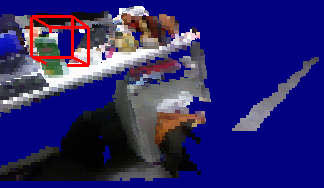
\includegraphics[width=.45\columnwidth]{figures/colorCHLAC/detection7.png}
\hfill
    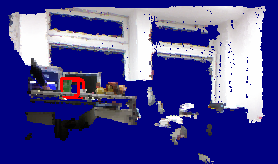
\includegraphics[width=.45\columnwidth]{figures/colorCHLAC/detection5.png} \\
\hfill
    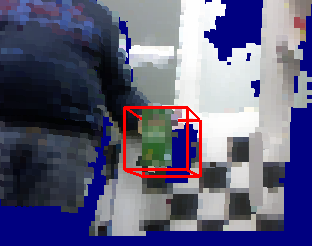
\includegraphics[width=.9\columnwidth]{figures/colorCHLAC/detection2.png}
\caption{An example of the detection of tetrahedral package of milk}
    \label{fig:milk_testing}
  \end{center}
\end{figure}


\section{Conclusions and Future Work}
\label{sec:conclusion}
\todo{ALL}

\section*{Acknowledgments}
CoTeSys
\todo{Asako: Dow we need to ack someone from ISI Lab}
%% Use plainnat to work nicely with natbib. 

\bibliographystyle{plainnat}
\bibliography{references}

\end{document}


%TODO:
%Check the original template and see what the meant with the hyperlinks
